One lasting scientific legacy of the {\it Hubble Space Telescope
(HST)} is the discovery of massive black holes at the centers of a
substantial fraction of galaxies, confirming the longstanding theory
of the ``central engines'' of quasars.  One of the major surprises
from the {\it Hubble} was the discovery of a strong correlation
between black hole mass and host galaxy
properties.\footnote{Assessment of Options for Extending the Life of
the Hubble Space Telescope: Final Report (2005);
https://www.nap.edu/read/11169/chapter/5).}  This connection, causal
or otherwise, may provide crucial clues to how and why these black
holes formed and how their host galaxies evolved. {\it As of the
launch of the James Webb Space Telescope (JWST), the question of how
black holes affect their host galaxies is one of the outstanding
questions in astrophysics.}

\smallskip \smallskip
\noindent
Observational and theoretical work now suggests that active galaxies
and black holes are potentially linked to both the triggering, and
``quenching'', of massive star formation. The link between massive
galaxies and their central super-massive black holes (SMBHs) that appear
ubiquitous is vital to the understanding of galaxy formation and
evolution, and significant observational and theoretical effort has
been invested in trying to measure and understand the physics involved
in these systems.  

\smallskip \smallskip
\noindent
The ``quenching'' of galaxy-wide star formation is supposedly driven
by `` AGN feedback'', where the AGN heats the surrounding gas corona,
offsetting cooling losses and disrupting the gas inflow. This feedback
manifests itself as high-velocity outflows from the AGN.  {\it However,
strong, direct observational evidence for AGN feedback is still lacking,
especially for the most luminous systems at $z=2-3$, at the height of
the Quasar Epoch.}  We have identified the best candidates that would
possess quasar feedback in action, in situ at high-redshift. These are
the ``Extremely Red Quasars'' identified via their WISE W3/4 colors.
As such, these mJy luminous AGN {\it are ideal targets for JWST MIRI}.


\section*{The Extremely Red Quasar Population} 
{\it Extremely Red Quasars (ERQs) are a unique obscured quasar
population with extreme physical conditions related to powerful
outflows across the line-forming regions. These sources are the
signposts of the most extreme form of quasar feedback at the peak
epoch of galaxy formation, and may represent an active ``blow-out''
phase of quasar evolution.}

\smallskip
\smallskip
\noindent
By matching the quasar catalogues of the Sloan Digital Sky Survey
(SDSS) and the Baryon Oscillation Spectroscopic Survey (BOSS) to the
Wide-Field Infrared Survey Explorer (WISE), Ross et al. (2015)
discovered quasars with extremely red infrared-to-optical colors:
$r_{\rm AB}-W4_{\rm Vega}>14$ mag, i.e., $F_\nu({\rm 22\mu
m})/F_\nu(r) \gtrsim 1000$; see Figure 1. These objects have infrared
luminosities $\sim$10$^{47}$ erg s$^{-1}$, and this initial study
returned a heterogeneous population, spanning a wide redshift range
$0.28 < z < 4.36$.

\smallskip
\smallskip
\noindent
Hamann et al. (2017) refined the selection of the ERQs, honing the
definition based on additional analysis and common properties, and
found more objects in this new scheme; a core sample of 97
ERQs with nearly uniform peculiar properties selected via \imw\ $\ge
4.6$ (AB) and REW(\civ ) $\ge$ 100 \AA\ at redshifts 2.0--3.4.  The
core ERQs have median luminosity $\left<\log L ({\rm ergs/s})\right>
\sim 47.1$, sky density 0.010 deg$^{-2}$, surprisingly flat/blue UV
spectra given their red UV-to-mid-IR colors, and common outflow
signatures including BALs or BAL-like features and large \civ\
emission-line blueshifts.  They have a suite of peculiar emission-line
properties including large rest equivalent widths (REWs), unusual
``wingless'' line profiles, large \nv /\lya , \nv /\civ , \siiv /\civ\
and other flux ratios, and very broad and blueshifted \oiii\ \lam 5007
(e.g., Figure~1, top right).  Their SEDs (Figure~\ref{fig:ERQ_SED},
{\it left}) and line properties are inconsistent with normal quasars
behind a dust reddening screen. Patchy obscuration by small dusty
clouds could produce the observed UV extinctions without substantial
UV reddening.


\hspace{-7.5cm}
\begin{figure}[h]
  \begin{center}
    \hspace{-0.5cm}
    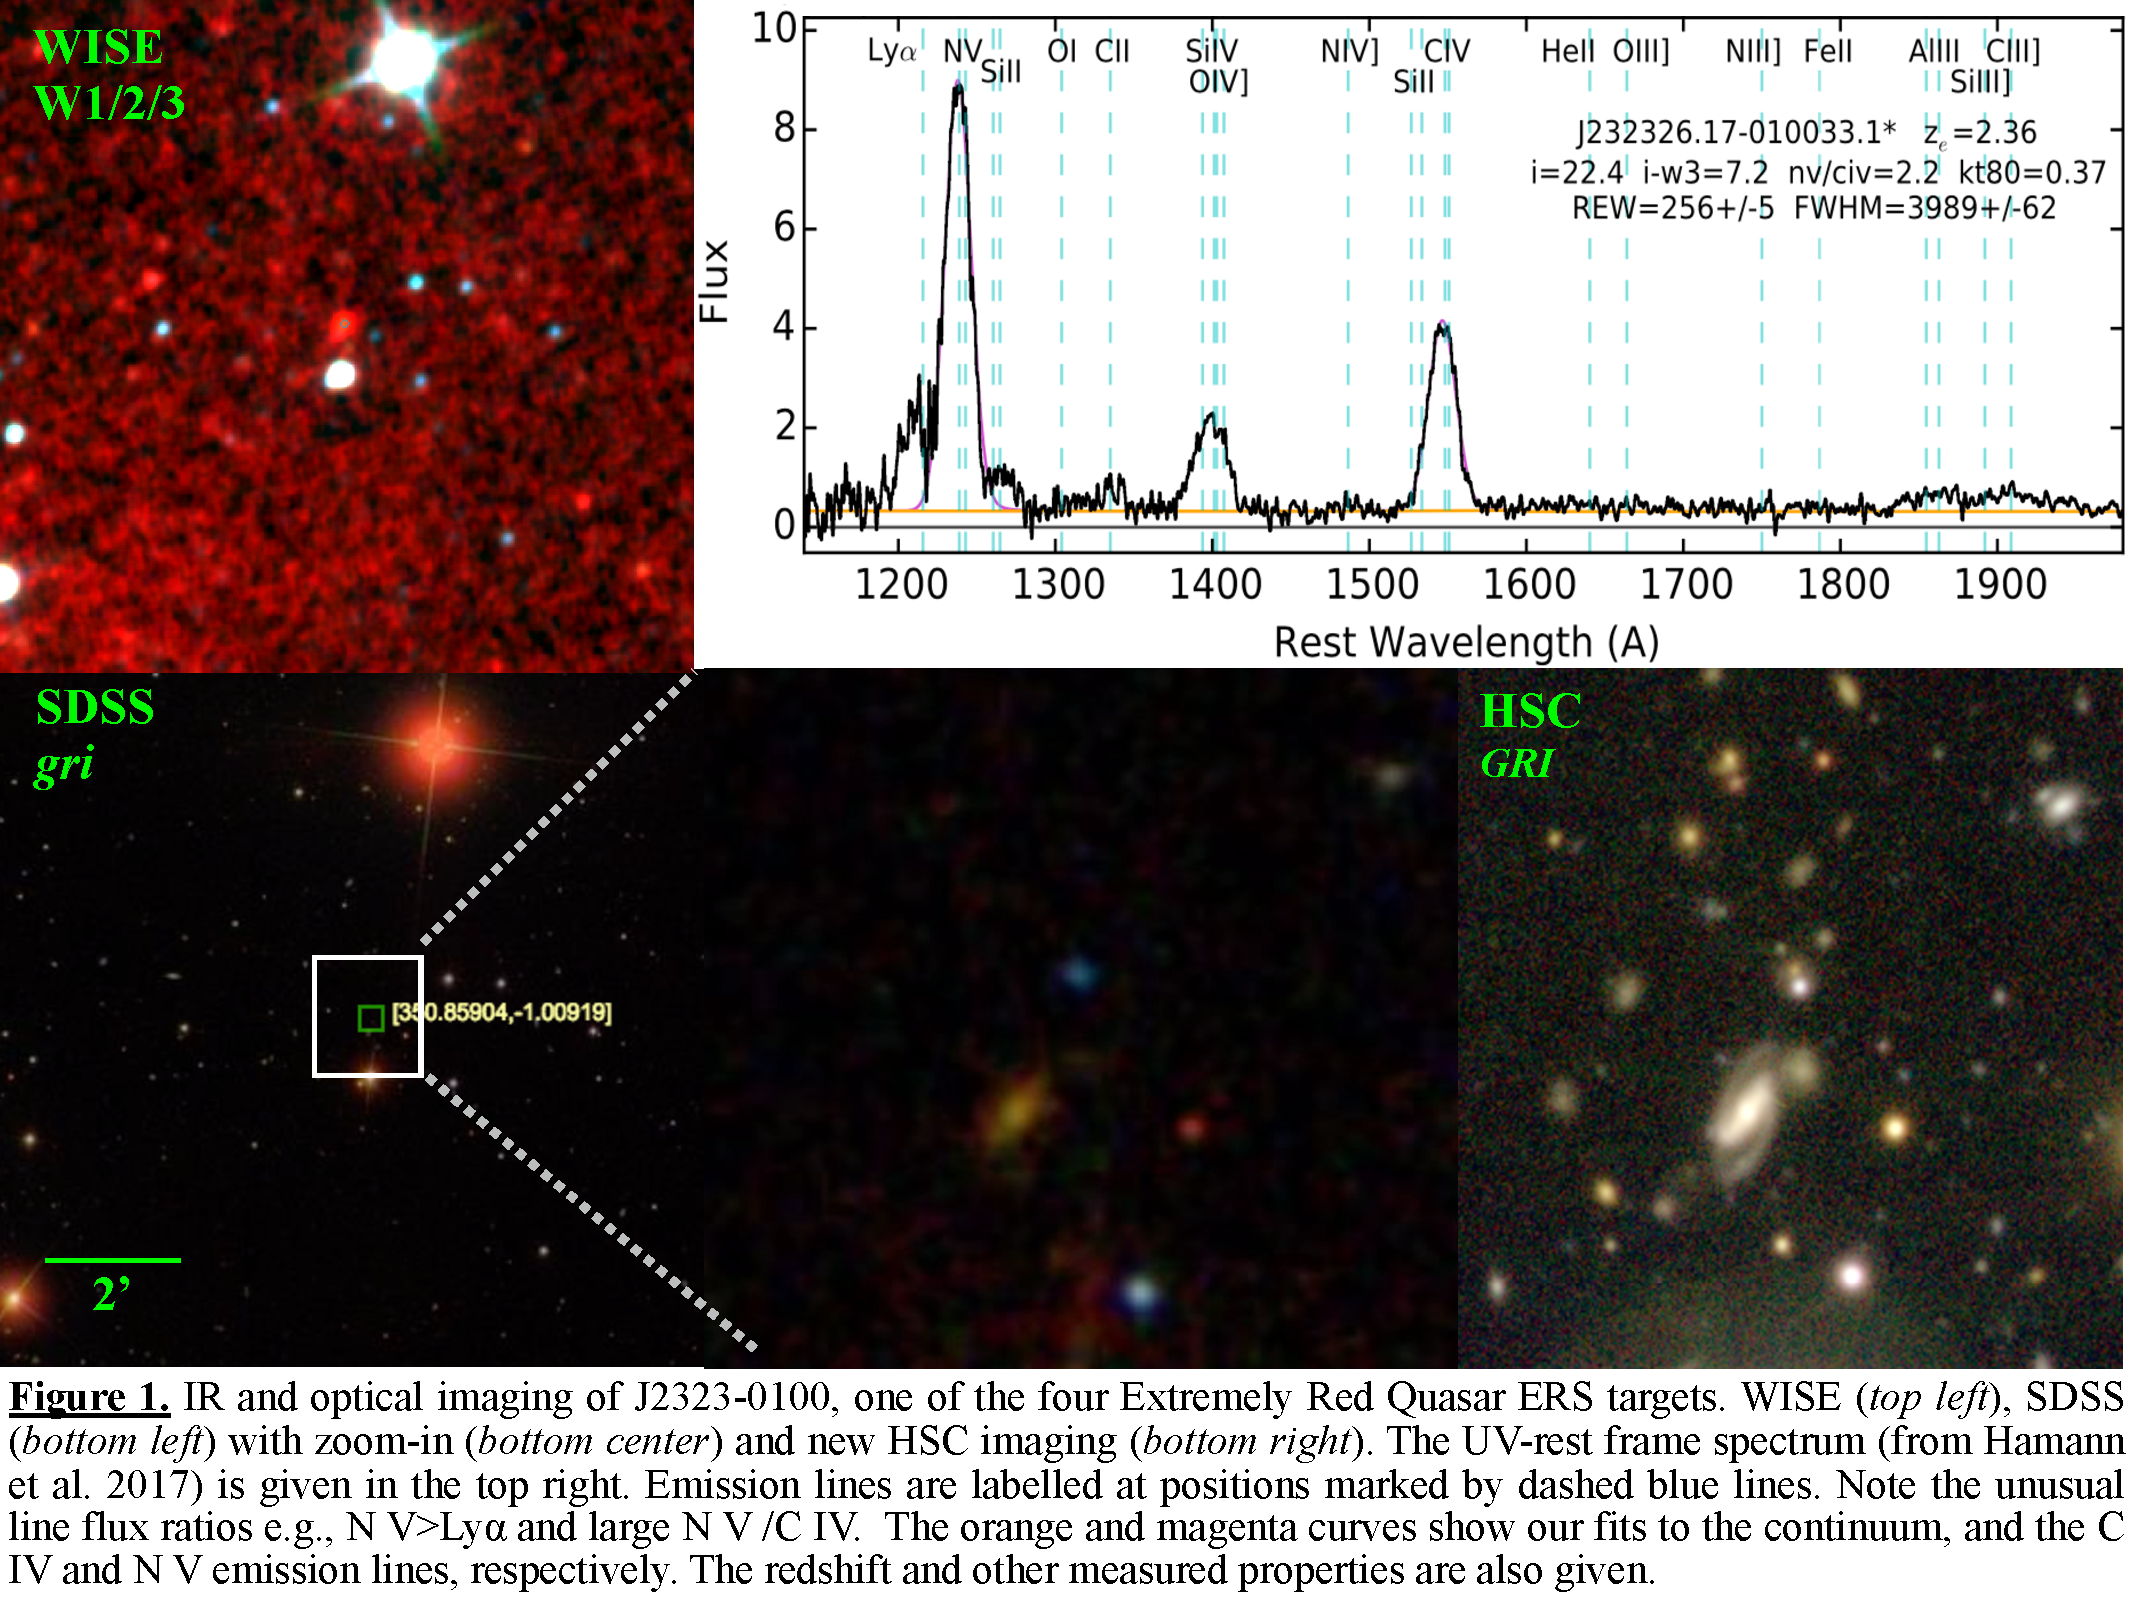
\includegraphics[height=12.0cm,width=16.0cm]{../Figures/WISE_SDSSzoomHSC_ERQ-image_v2.pdf}
    \vspace{-10pt}
    \vspace{-14pt}
    \label{figtest-fig}
  \end{center}
\end{figure}

\setcounter{figure}{1}
\hspace{-2.5cm}
\begin{figure}[h]
  \begin{center}
    \hspace{-0.5cm}
% trim=l b r t
    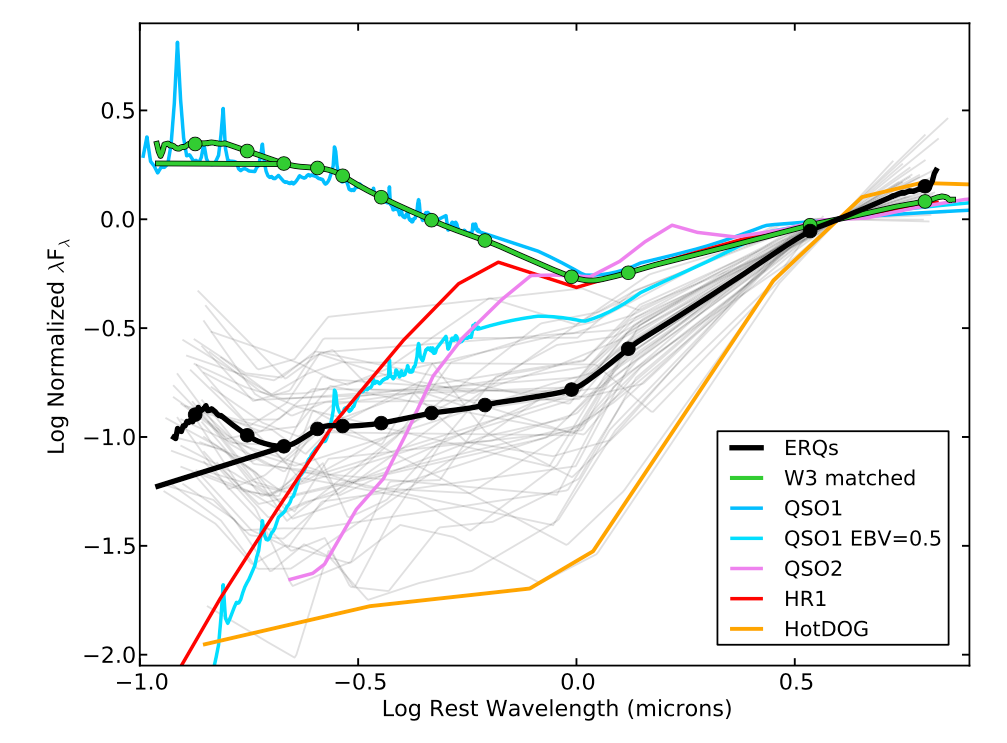
\includegraphics[height=7.0cm,width=7.2cm,  trim={42pt 0pt 22pt 12pt},clip]{../Figures/Hamann2017_Fig16_SEDs.png}
    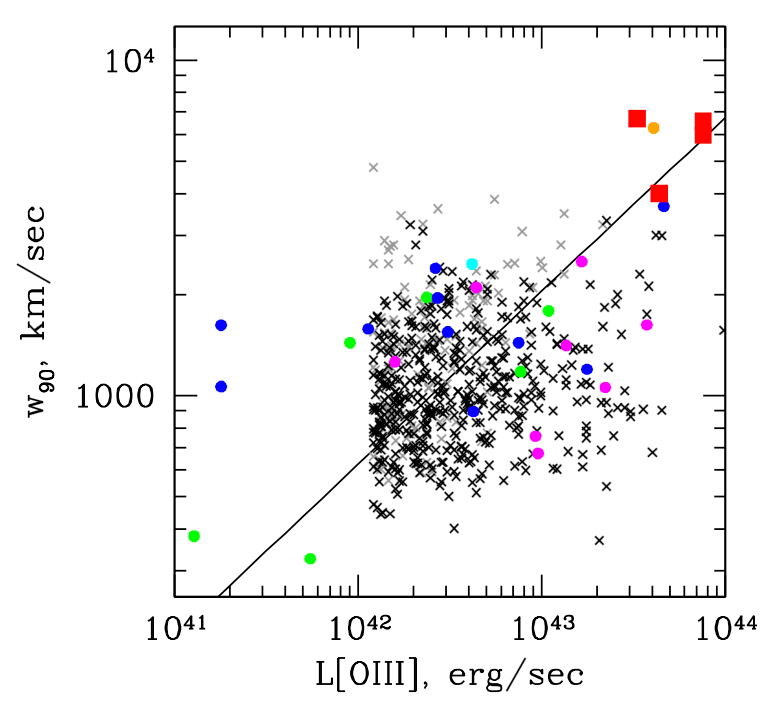
\includegraphics[height=7.1cm,width=7.4cm, trim={12pt 22pt 42pt 12pt},clip]{../Figures/Zakamska_2016_Fig9.png}
    \vspace{-10pt}
    \caption{
      % \small
      %\footnotesize
      \scriptsize
      % \tiny
      {\it (Left)} From Hamann et al., 2017, the normalized median
      SEDs for Type 1 non-BALs in the core ERQ sample (black curve) plus
      blue quasars matched to the core ERQs in W3 magnitude (green curve).
      The Type 1 quasar template with and without reddening equal to $E(B-V)
      = 0.5$ (light blue, `QSO1', from Polletta et al. 2007), a typical Type
      2 quasar from Mateos et al. (2013; `QSO2', purple), a typical heavily
      reddened Type 1 quasar from Banerji et al. (2013; `HR1'), and a
      typical HotDOG from Tsai et al. (2015). The light grey curves are SEDs
      of individual core ERQs.
      %%
      {\it (Right)} \oiii\ kinematics as a function of luminosities
      for our four targets, red squares, with other quasar populations are
      shown by black points and various colored symbols.  At these extreme
      velocities, the gas cannot be confined by any realistic galaxy
      potential and is thus likely to escape from the galaxy; these objects
      are likely signposts of the extreme `blow-out' phase of quasar
      feedback observed at the peak epoch of galaxy formation.
    }
    \vspace{-14pt}
    \label{fig:ERQ_SED}
  \end{center}
\end{figure}
\vspace{-22pt}

\smallskip
\smallskip
\noindent
Further observations by our team with VLT/XShooter measured rest-frame
optical spectra of four of the $z\sim 2.5$ ERQs (Zakamska et al. 2016)
which revealed very broad (FWHM = 2600-5000 km s$^{-1}$), strongly
blue-shifted (by up to 1500 km s$^{-1}$) \oiii\ $\lambda$5007\AA\
emission lines in these objects. In a large sample of type 2 and red
quasars, \oiii\ kinematics are positively correlated with infrared
luminosity, and the four objects in our sample are on the extreme end
both in \oiii\ kinematics and infrared luminosity.  As such, we
estimate that at least 3\% of the bolometric luminosity in these
objects is being converted into the kinetic power of the observed
wind. Photo-ionization estimates suggest that the \oiii\ emission
might be extended on a few kpc scales, which would suggest that the
extreme outflow is affecting the entire host galaxy of the quasar.
%% [Ne V] 14.3, 24.2 μm 97.
%% [Ne II] 12.8 μm
%% [OIV] 26μm


\begin{SCfigure}
  \centering
  %% trim=l b r t
  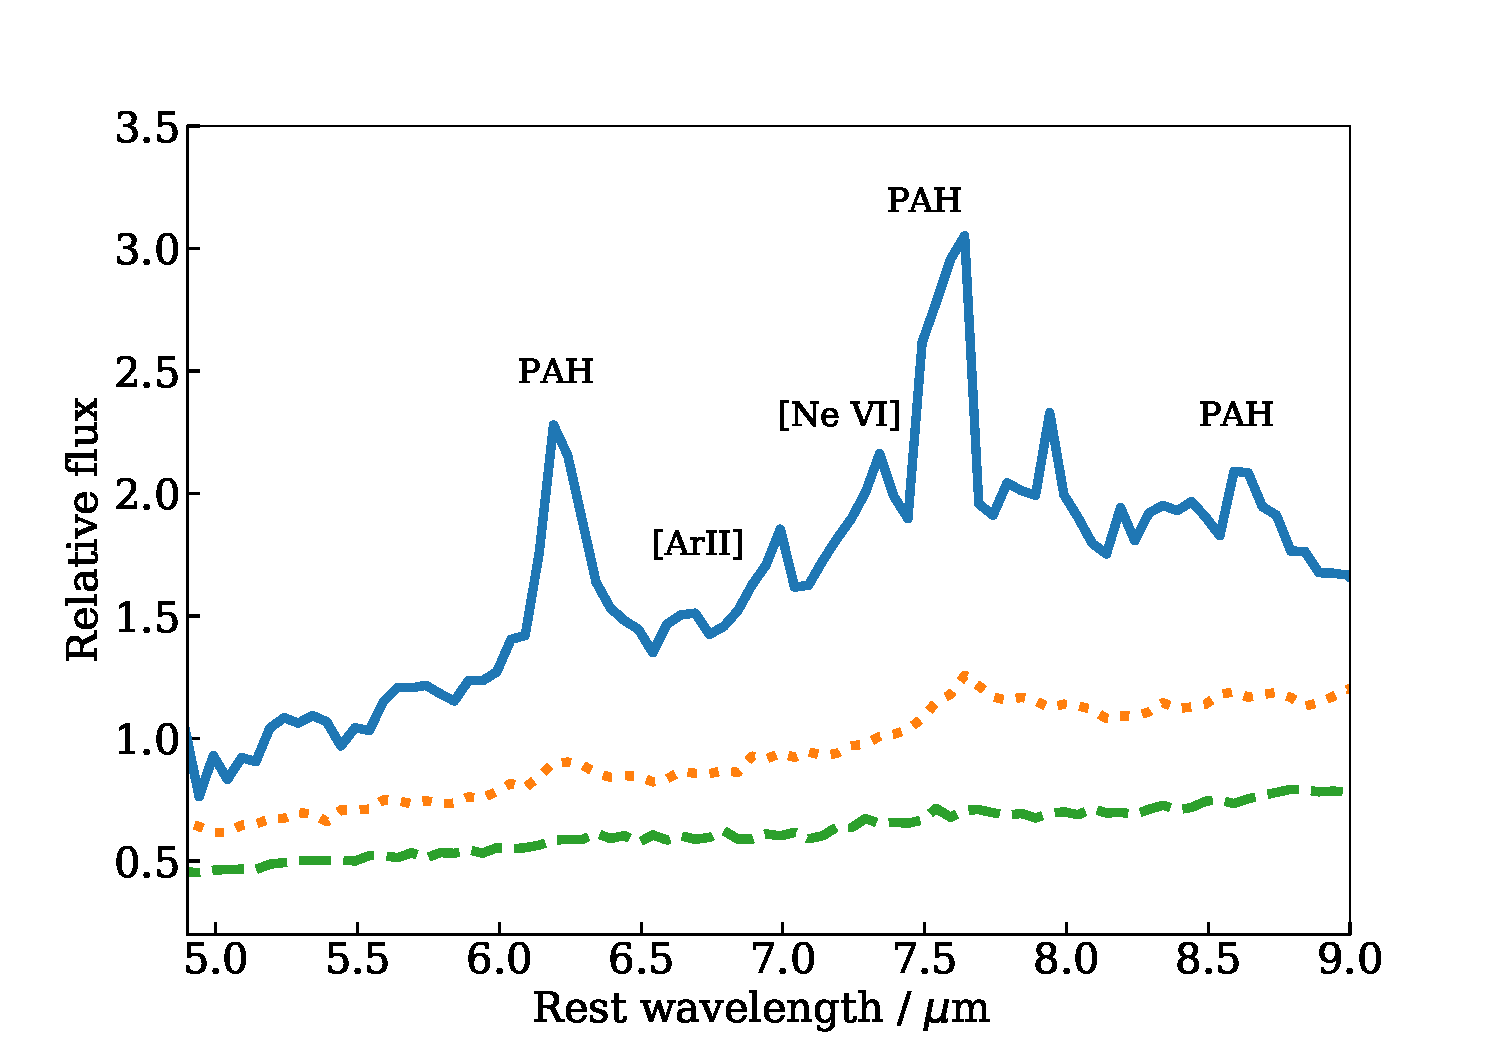
\includegraphics[height=7.0cm,width=9.5cm, trim={32pt 6pt 42pt 12pt},clip]{../Figures/Hill2014_IRspectra_Lrange_v2}
  % \small \footnotesize \scriptsize \tiny
  \caption{\footnotesize    
    Example {\it Spitzer} IRS composite spectra, from Hill et al. (2014). 
    Each composites has 61 quasars, in the luminosity
    ranges log $L_{5.6}$ =41.0-43.6 (blue solid), 43.6-44.7 (orange dotted) 
    and 44.8-46.1 (green dashed). 
    %These   templates are low resolution and do not cover $\lambda<5\mu$m. 
    With
    {\it Spitzer} summing composites was necessary to see the spectral
    features; with {\it JWST} MIRI MRS we will be able to see these features
    in individual AGN. Our null hypothesis is that the dominant emission
    is from the AGN, but this has never been tested at our redshift or IR
    luminosity.}
  \label{fig:eg_spectra}
\end{SCfigure}
\normalsize

\smallskip
\smallskip
\noindent
{\bf \underline{MIR spectroscopy and PAHs}:}
Polycyclic Aromatic Hydrocarbons (PAHs) are abundant, ubiquitous, and
dominate the structure and evolution of the ISM of galaxies.  Aromatic
features are already a significant component of dusty galaxy spectra
as early as $z\approx2$, and the infrared (IR) emission features at
3.3, 6.2, 7.7, 8.6, and 11.3 $\mu$m are generally attributed to IR
fluorescence from (mainly) far-ultraviolet (FUV) pumped large PAH
molecules. {\it As such, these features trace the FUV stellar flux and
are thus a measure of star formation.} The interstellar IR emission
spectrum is incredibly rich and shows a wealth of detail. {It is
dominated by major PAH emission features at 3.3, 6.2, 7.7 and 8.6
$\mu$m.  In addition, there are weaker features at 3.4, 3.5, 5.25,
5.75, 6.0, 6.9 and 7.5$\mu$m. {\it Given the redshift of our ERQs and
the MIRI wavelength coverage we will cover $1.36 \leq \lambda_{\rm
emitted} \leq 8.6 \mu$m.}  In theory, we can detect the 3$\mu$m and
6.0$\mu$m water-ice feature, and figure out {\it where} it is most
prevalent in the quasar. Figure~\ref{fig:eg_spectra} shows an example
of the current state-of-the-art in quasar MIR spectral composites with
$\approx$60 {\it Spitzer} IRS quasars per bin.  {\it We will have
equivalent SNR from 1 quasar, across a broader wavelength range and in
a new redshift-luminosity regime.}

\smallskip
\smallskip
\noindent
The mid-IR spectral region also presents a suite of high-ionization
lines: \snine\ at 1.252$\mu$m, \six\ at 1.430$\mu$m, \sixi\ at
1.932$\mu$m, \sivi\ at 1.962$\mu$m, \caviii\ at 2.321$\mu$m, \sivi\ at
2.483$\mu$m \siix\ at 3.935$\mu$m and \arii\ at 6.97$\mu$m.  However,
most critically, we have access to the \nevi\ line at 7.65$\mu$m,
which with an ionization potential of 158 eV is much too high for
stars.  {\bf The [Ne VI] 7.65$\mu$m line can be used to measure the
instantaneous luminosity of the central engine.}  [Ne VI] 7.65$\mu$m
has a critical density of $\sim10^{6}$ cm$^{-3}$ and very low
interstellar extinction.  Its ratio to the hydrogen recombination
lines is almost independent of ionization parameter thus making this a
superb emission line to utilize.

\smallskip
\smallskip
\noindent
{\it With the IFU spatial information, at medium resolution, we will
be able to (i) map the PAH emission structure of the extremely red
quasars on sub-kiloparsec scales and (ii) look for offsets in these
emissions that could well be indicative of `AGN feedback'.}

\smallskip
\smallskip
\noindent
{\bf \underline{Integral Field Unit Observations:}} 
The ability for the MRS to obtain integral field unit spectroscopy
allows us to investigate the {\it spatial information} associated with
the high IR fluxes in the ERQs. The spatial distribution of the IR
will give direct clues to the power source of the IR emission.  The
IFU aspect of the Medium Resolution Spectrometer will allow
investigations in unprecedented detail of both the central AGN IR
emission and any potentially extended emission in $z\approx2.5$
quasars.  As a null hypothesis, we suggest that weak PAH emission will
be in the nuclear regions and strong(er) PAH emission in the extended
source. However, very recent studies with H$\alpha$ of $z\sim2$
quasars suggest that narrow H$\alpha$ emission might be from a
spatially unresolved source.

\smallskip \smallskip
\noindent 
Our final primary science goal will be to examine the IR spectral
emission lines (PAH or high ionization) and place them in context with
the host galaxy by looking for emission line offsets or blends.
The kinematics of the \oiii\ $\lambda \lambda$4959,5007 \AA\ emission
lines are {\it known to be extreme} in these objects, being very broad
(FWHM=2600--5000 km s$^{-1}$) and strongly blueshifted (by up to 1500
km s$^{-1}$; Figure 2, {\it right}). We also know that the \oiii\
kinematics are positively correlated with infrared luminosity.  Can we
place the PAH and AGN emission in the same consistent kinematic
structure?  Is there a spatial variation of the kinematics of the IR
emission lines, and if so, is it consistent with a strong `AGN
feedback' phase?

\smallskip \smallskip
\noindent 
{\it Given the pixel scales of the MRS IFU, and the fact that 1'' is $\approx$8 kpc 
at $z\sim2.5$ a major challenge, goal and SEP will be to deliver 
software and analyses that samples the data on a sub-pixel scale.}


%\medskip \medskip \medskip \medskip
%\clearpage


